% Week 10: curvature shapes (FPCA) in the pLAD and mLAD, explained on made-up data. Input from week10.tex.
% Figures: fpca_steps_figures.py. Text left, figure right (minipages, so no extra package is needed).
\newcommand{\fpcarow}[2]{\par\noindent
  \begin{minipage}[t]{0.54\textwidth}\vspace{0pt}#1\end{minipage}\hfill
  \begin{minipage}[t]{0.42\textwidth}\vspace{0pt}#2\end{minipage}\par\medskip}
\newcommand{\fpcafig}[2]{\centering\includegraphics[width=\linewidth]{week_figure/fpca_steps/fake/#1}\\[-0.1em]
  {\footnotesize #2}}

\subsection*{Curvature shapes in the proximal and mid LAD (FPCA)}
In the main model, curvature is the mean turning of each segment. The mean does not say where the
vessel bends: one sharp bend and a gentle turn along the whole segment can give the same mean.
Functional principal component analysis (FPCA) finds the few main shapes in which people's turning
differs along a segment, and gives each person a score for how much of each shape they have. These
scores then replace the mean in the risk model, to see whether where the vessel bends matters, not
only how much. This is only done in the pLAD and mLAD, the only segments where enough people developed
plaque to estimate several curvature terms, and it is descriptive. The figures use made-up people.

\fpcarow{%
\textbf{Turning angle.} At each point of the centerline, one point is placed 5\,mm before it and one
5\,mm after it, in a straight line. The turning angle is the angle between the line coming in and the
line going out: how much the vessel changes direction at that point. Dividing it by the 5\,mm gives the
turning in rad/mm. Bends shorter than about 5\,mm are not seen, and the first and last 5\,mm of a
vessel get no value. It is computed along the whole
artery and then cut at the segment boundaries, so a bend across a boundary is still measured.
}{%
\centering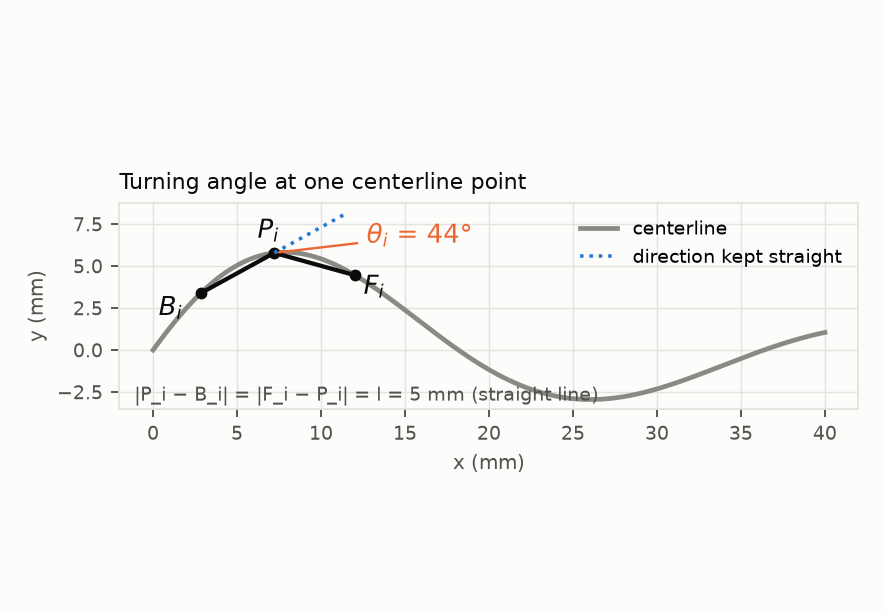
\includegraphics[width=\linewidth]{week_figure/fpca/f1_turning_geometry.png}\\[-0.1em]
{\footnotesize The turning angle $\theta_i$ at one point of a made-up centerline.}
}

\fpcarow{%
\textbf{The same 50 places for everyone.} The turning has one value per centerline point, and
segments differ in length and in how many points they have (top). To compare people place by place,
each segment is stretched or squeezed to run from 0 (start) to 1 (end), and the turning is read at the
same 50 places (bottom). Place 25 is then halfway along the segment for everyone, whether the segment
is 30 or 50\,mm long. The shapes therefore describe
where along the segment the vessel turns, not how long it is.
}{%
\centering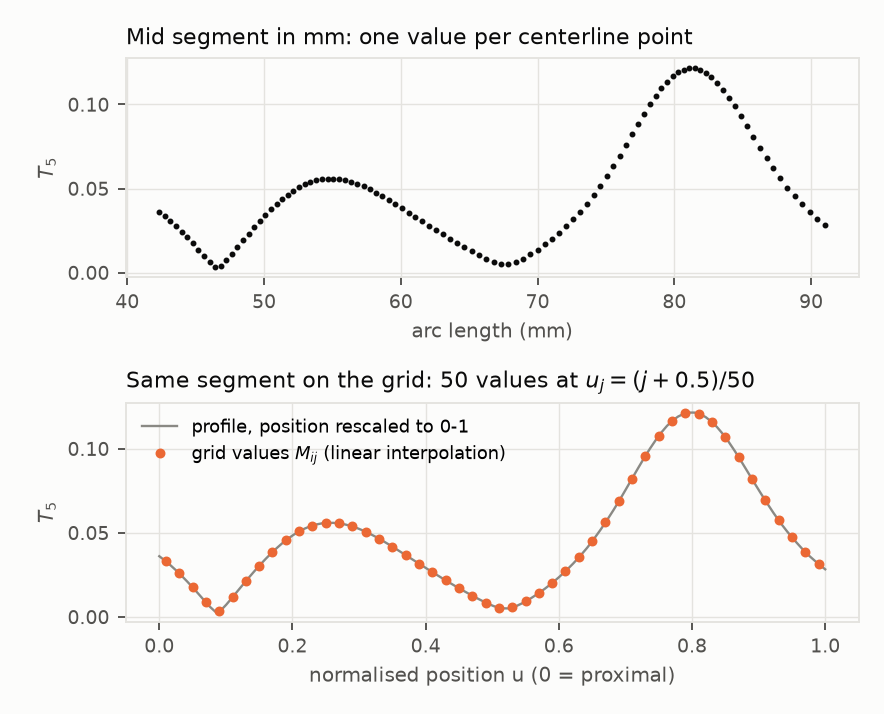
\includegraphics[width=\linewidth]{week_figure/fpca/f3_grid.png}\\[-0.1em]
{\footnotesize One made-up segment in mm (top) and read at the 50 places (bottom).}
}

\fpcarow{%
\textbf{Turning curves and deviations.} Each person is now one curve of 50 values (top, grey). The average curve (black) says how much everybody turns at
each place, for example that everybody turns more near the start. It is the same for everyone, so it
cannot tell people apart. At each place the average there is subtracted from everyone. What is left,
the deviation (bottom), is how much and where each person turns more or less than the average person. Where the bundle is wide, people
differ a lot. A bend covers several neighbouring places, so these places go up and down together
across people; FPCA looks for such groups of places, and each group becomes a shape.
}{%
\fpcafig{f4_profiles_deviations.png}{Turning curves of made-up people with their average (top), and
the same curves minus the average (bottom).}
}

\fpcarow{%
\textbf{Shapes, one at a time.} The first shape is the pattern along which people differ most (top
left). Each person has some amount of it, their score, and when that amount is taken away, less of the
differences is left (top right). The next shape is found in what is left, and so on, so each shape
describes something the earlier ones do not. Here the first shape is almost flat and positive, and
the next shapes say \emph{where} a person turns: more at the start than at the end, or more in the
middle than at the ends.

\medskip
\textbf{Number of shapes.} After the real shapes, new shapes only describe noise. Three checks decide
where to stop: whether a shape explains more than it would by chance, whether it comes back when the
people are redrawn, and how many shapes best predict a hidden part of a curve. The smallest of the
three is used, and it is fixed before plaque is looked at, so the choice cannot be tuned to find an
effect.
}{%
\fpcafig{f6_steps.png}{Left: what is not yet explained, with the next shape. Right: what is left.}
}

\textbf{A flat first shape is the mean turning.} The first shape is the main way in which people's
curves differ. When it is flat, that difference is the same all along the segment: a person who turns
more than average at the start also tends to turn more than average in the middle and at the end, by
about the same amount. Drawn as the average plus and minus the shape, it gives two curves parallel to
the average, one above and one below. The largest difference between people is then not \emph{where}
they bend but \emph{how much} they bend overall, which is exactly what the mean turning measures. Here
the first shape is only nearly flat, yet the score on it and the mean turning correlate 0.998.

\textbf{We see the same in the Herlev--{\O}sterbro data.} In the Medis centerlines the first shape has
the same sign along the whole segment and is close to a straight line, and explains the largest
share of the differences, so the mean turning captures most of what separates them.
The Medis trees come from participants with plaque at baseline, so this must be confirmed in the
plaque-free cohort.
\par\medskip

\fpcarow{%
\textbf{From scores to the risk model.} The shapes are the same for everyone; a person's score says
how much of a shape they have. It is found by comparing the person's curve with the shape at every
position: the more they match, the higher the score. A person who follows the shape gets a positive
score, one who does the opposite a negative score, and the average person 0. The average plus each
shape times its score rebuilds the curve (top), so a few scores replace the 50 numbers and go into the
risk model of the segment, next to SCORE2:
\[
  \mathrm{cloglog}(p_i) = a + g\,\mathrm{SCORE2}_i + \sum_{k} b_k\, z_{ik},
\]
where $p_i$ is the risk that person $i$ develops plaque in the segment and $e^{b_k}$ the hazard ratio
per SD of shape $k$. The weights read back as one weight per place (bottom). They are not estimated
yet, so which parts of each shape raise or lower the risk is unknown.
}{%
\centering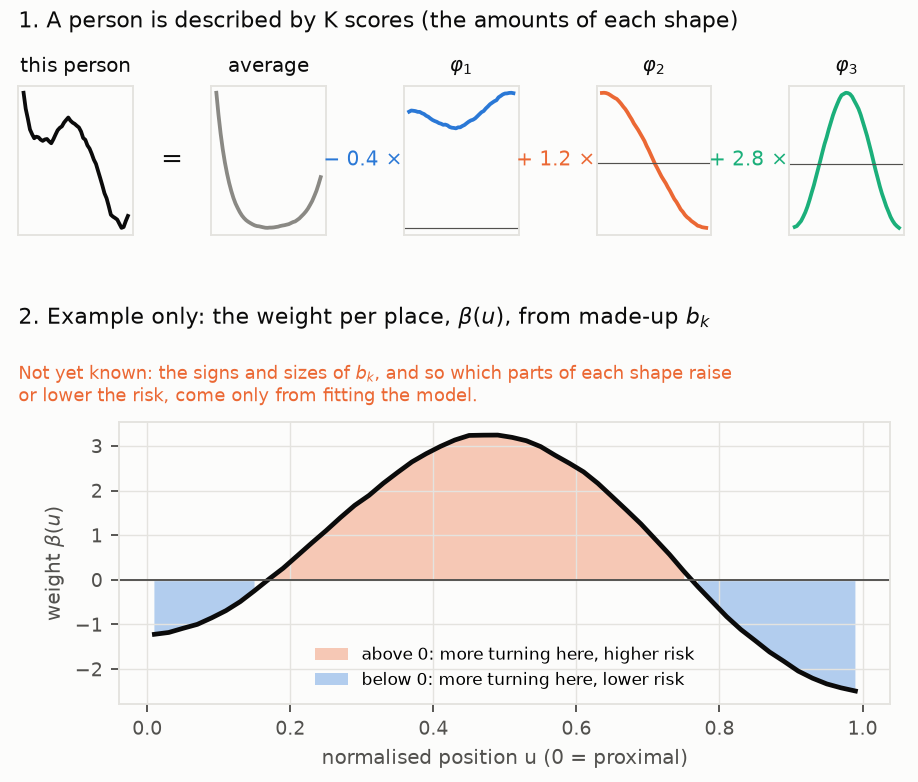
\includegraphics[width=0.88\linewidth]{week_figure/fpca_steps/fake/p3_story.png}\\[-0.1em]
{\footnotesize Top: one made-up person as the average plus scores times shapes. Bottom: made-up
weights; the real signs are not yet known.}
}

\textbf{The end goal.} The aim is to see whether some patterns of turning carry more risk than others,
that is, whether the weights of some shapes have more predictive value than others. A person who turns
a lot at the start of the segment and hardly at all after it may carry more risk than a person who
turns a little the whole way along, even with the same mean turning, and the mean turning cannot tell
these two apart. The main model keeps the mean turning: it was chosen beforehand, as earlier studies
point to it and it explains most of the differences between people, and it is not changed after this
analysis, to avoid choosing the model by its p-values.
